% Options for packages loaded elsewhere
\PassOptionsToPackage{unicode}{hyperref}
\PassOptionsToPackage{hyphens}{url}
\PassOptionsToPackage{dvipsnames,svgnames,x11names}{xcolor}
\documentclass[
  11pt,
]{article}
\usepackage{xcolor}
\usepackage[margin=2.4cm]{geometry}
\usepackage{amsmath,amssymb}
\setcounter{secnumdepth}{-\maxdimen} % remove section numbering
\usepackage{iftex}
\ifPDFTeX
  \usepackage[T1]{fontenc}
  \usepackage[utf8]{inputenc}
  \usepackage{textcomp} % provide euro and other symbols
\else % if luatex or xetex
  \usepackage{unicode-math} % this also loads fontspec
  \defaultfontfeatures{Scale=MatchLowercase}
  \defaultfontfeatures[\rmfamily]{Ligatures=TeX,Scale=1}
\fi
\usepackage{lmodern}
\ifPDFTeX\else
  % xetex/luatex font selection
\fi
% Use upquote if available, for straight quotes in verbatim environments
\IfFileExists{upquote.sty}{\usepackage{upquote}}{}
\IfFileExists{microtype.sty}{% use microtype if available
  \usepackage[]{microtype}
  \UseMicrotypeSet[protrusion]{basicmath} % disable protrusion for tt fonts
}{}
\usepackage{setspace}
\makeatletter
\@ifundefined{KOMAClassName}{% if non-KOMA class
  \IfFileExists{parskip.sty}{%
    \usepackage{parskip}
  }{% else
    \setlength{\parindent}{0pt}
    \setlength{\parskip}{6pt plus 2pt minus 1pt}}
}{% if KOMA class
  \KOMAoptions{parskip=half}}
\makeatother
\usepackage{longtable,booktabs,array}
\newcounter{none} % for unnumbered tables
\usepackage{calc} % for calculating minipage widths
% Correct order of tables after \paragraph or \subparagraph
\usepackage{etoolbox}
\makeatletter
\patchcmd\longtable{\par}{\if@noskipsec\mbox{}\fi\par}{}{}
\makeatother
% Allow footnotes in longtable head/foot
\IfFileExists{footnotehyper.sty}{\usepackage{footnotehyper}}{\usepackage{footnote}}
\makesavenoteenv{longtable}
\usepackage{graphicx}
\makeatletter
\newsavebox\pandoc@box
\newcommand*\pandocbounded[1]{% scales image to fit in text height/width
  \sbox\pandoc@box{#1}%
  \Gscale@div\@tempa{\textheight}{\dimexpr\ht\pandoc@box+\dp\pandoc@box\relax}%
  \Gscale@div\@tempb{\linewidth}{\wd\pandoc@box}%
  \ifdim\@tempb\p@<\@tempa\p@\let\@tempa\@tempb\fi% select the smaller of both
  \ifdim\@tempa\p@<\p@\scalebox{\@tempa}{\usebox\pandoc@box}%
  \else\usebox{\pandoc@box}%
  \fi%
}
% Set default figure placement to htbp
\def\fps@figure{htbp}
\makeatother
\setlength{\emergencystretch}{3em} % prevent overfull lines
\providecommand{\tightlist}{%
  \setlength{\itemsep}{0pt}\setlength{\parskip}{0pt}}
\usepackage{amsmath,amssymb}
\usepackage{booktabs}
\usepackage{float}
\floatplacement{figure}{H}
\usepackage{bookmark}
\IfFileExists{xurl.sty}{\usepackage{xurl}}{} % add URL line breaks if available
\urlstyle{same}
\hypersetup{
  pdftitle={Tree--network distinguishability fails under the Kimura two-parameter model},
  pdfauthor={Anonymous},
  colorlinks=true,
  linkcolor={Maroon},
  filecolor={Maroon},
  citecolor={Blue},
  urlcolor={Blue},
  pdfcreator={LaTeX via pandoc}}

\title{Tree--network distinguishability fails under the Kimura
two-parameter model}
\usepackage{etoolbox}
\makeatletter
\providecommand{\subtitle}[1]{% add subtitle to \maketitle
  \apptocmd{\@title}{\par {\large #1 \par}}{}{}
}
\makeatother
\subtitle{Exact counterexamples and a classification of trinets up to
level three}
\author{Anonymous}
\date{5 October 2026}

\begin{document}
\maketitle
\begin{center}Unrefereed candidate, version 1.1.0\\ DOI: \href{https://doi.org/10.5281/zenodo.23165616}{10.5281/zenodo.23165616}\end{center}

\setstretch{1.12}
\subsection{Abstract}\label{abstract}

Brits, Holtgrefe, van Iersel and Martin (2026) proved that, under the
Jukes--Cantor (JC) model of nucleotide substitution, no phylogenetic
network containing a non-trivial blob with three or more outgoing edges
produces the same leaf-pattern distribution as a phylogenetic tree.
Their parameter space consists of stochastic, positive-definite
transition matrices with non-trivial reticulation weights. Whether the
same holds for the Kimura two-parameter (K2P) model was left open; an
earlier version of their paper asserted it, and the assertion was
withdrawn. This note shows that the extension is false.

A three-leaf network with two reticulations, whose internal graph is the
complete bipartite graph \(K_{2,3}\), has exactly the 64-entry
leaf-pattern distribution of a three-leaf star tree for an explicit
choice of rational network parameters. Every edge matrix of both models
comes from an edge-specific continuous-time K2P process in which the
transition rate exceeds the transversion rate. On the larger stochastic
parameter space, precisely the three unstacked level-two trinets have
models intersecting the tree model; only the \(K_{2,3}\) seed is
certified here under continuous-time, transition-biased parameters. A
separate convexity argument excludes its coincidence when both models
must share the same prescribed rate ratio greater than one.

The positive cases are explained by an \emph{anchoring} condition, under
which the JC induction of Brits et al.~remains tied to a single leaf;
anchored networks of any level are distinguishable from trees. For
networks of level at most three the condition is also necessary: 30 of
the 83 reduced level-3 three-leaf networks are anchored, and each of the
other 53 coincides with a tree. The coincidences extend to networks with
any number of leaves, to every level of at least two, and to the Kimura
three-parameter (K3P) model. Every positive and negative claim for the
published parameter space rests on a proof or an exact-arithmetic
certificate. Two statements about the subset of continuous-time
parameters remain conjectural.

\subsection{1. The question}\label{the-question}

A phylogenetic network records reticulate events such as hybridisation
by allowing a vertex two parents. Under a Markov substitution model on a
network, each site evolves along one of the network's displayed trees,
chosen by independent coin flips at the reticulations, so the
leaf-pattern distribution is a mixture of tree distributions (Gross \&
Long, 2018; Brits et al., 2026). A basic requirement for inferring
reticulation from sequence data is that such mixtures cannot reproduce
the distribution of an ordinary tree.

Brits et al.~(2026) established this for the JC model. Their argument
has three parts. First, restriction to three leaves: if a network with a
non-trivial blob produced a tree distribution, so would some three-leaf
network (a \emph{trinet}) with a non-trivial three-blob. Second, a
\emph{trinet inequality}: the polynomial
\(q_{ACC}q_{CAC}q_{CCA} - q_{AAA}q_{TCG}^2\) in Fourier coordinates
vanishes on star trees and is strictly positive on every trinet with a
non-trivial three-blob. Third, the inequality is proved by induction on
the number of reticulations, splitting a trinet at a reticulation
adjacent to a leaf. The induction needs the polynomial to be symmetric
under permutations of the leaves, which holds for JC.

For K2P the same authors proved the level-1 case: the polynomial
\[Q = q_{AGG}\,q_{GAG}\,q_{CCA}^2 - q_{AAA}\,q_{GGA}\,q_{TCG}^2\]
vanishes on star trees and is strictly positive on every three-leaf
network with one reticulation adjacent to leaf 3 (their Lemma 4.1;
numbering of arXiv version 3). Versions 1 and 2 of the preprint extended
this to all levels. Version 3 withdrew the extension, noting that \(Q\)
is not symmetric under leaf permutations for K2P, so the induction
hypothesis need not apply to the smaller networks. The discussion of
version 3 lists as open whether the higher-level trinet inequality
extends to K2P and K3P.

The answer is negative, and not only because the proof fails: the
statement is false. Section 5 gives an exact counterexample; Sections
6--8 determine which trinets of level two and three are distinguishable
from trees, and show how the failures propagate to larger networks.

\subsection{2. Setting}\label{setting}

\subsubsection{2.1 Networks}\label{networks}

We follow the definitions of Brits et al.~(2026, Section 2). A
\emph{semi-directed} network is obtained from a binary rooted
phylogenetic network by suppressing the root and undirecting every edge
except the reticulation edges (the two edges entering each reticulation
vertex). A \emph{blob} is a maximal connected subgraph without cut
edges; an \(m\)-blob meets \(m\) edges outside itself. A \emph{trinet}
is a semi-directed network on three leaves. A \emph{2-sub-blob} is a set
\(W\) of at least two internal vertices inducing a connected subgraph
and joined to the rest of the network by exactly two edges; Brits et
al.~(2026, Lemma 5.1 and Corollary 5.2) show that suppressing
2-sub-blobs can only enlarge a model, so trinets without 2-sub-blobs
(\emph{reduced} trinets) are the cases that matter. A reduced trinet
with a non-trivial three-blob consists of that blob and three pendant
leaf edges; its level is its number of reticulations.

Deleting one of the two edges entering each reticulation leaves a
spanning tree, a \emph{displayed tree}. In the displayed-tree model each
reticulation \(h\) carries a weight \(\delta_h \in (0,1)\) for one of
its incoming edges and \(1-\delta_h\) for the other, and the network
distribution is the weighted mixture of the displayed trees'
distributions.

\subsubsection{2.2 The K2P model in Fourier
coordinates}\label{the-k2p-model-in-fourier-coordinates}

The root distribution is uniform on the four states. Edge parameters,
including transition/transversion ratios, may differ between edges.
Outside the stochastic region we use the term \emph{parameterised
Fourier model}, not probability distribution.

Identify the nucleotides with the Klein group
\(\mathbb{Z}_2\times\mathbb{Z}_2\) by \(A=(0,0)\), \(C=(0,1)\),
\(G=(1,0)\), \(T=(1,1)\). The transition matrix on an edge \(e\) is
\(M_e(u,v) = f_e(u+v)\), where
\[f(A)=\tfrac{1+2X+Y}{4},\qquad f(C)=\tfrac{1+Y-2X}{4},\qquad f(G)=f(T)=\tfrac{1-Y}{4}.\]
Its eigenvalues are \(1, X, Y, X\); in the notation of Brits et
al.~\(a^e_A=1\), \(a^e_C=a^e_T=X_e\) and \(a^e_G=Y_e\). The substitution
class \(u\mapsto u+C\) has its own probability and the other two classes
share one. Relabelling nucleotides so that this class becomes
\(A\leftrightarrow G\), \(C\leftrightarrow T\) gives Kimura's (1980)
model, and we call it the \emph{transition} class. In continuous time,
with rate \(\alpha\) for transitions and rate \(\beta\) for each of the
two transversion classes, an edge of length \(t\) has
\(X = e^{-2(\alpha+\beta)t}\) and \(Y = e^{-4\beta t}\).

Three nested parameter regions are used for each edge:

\begin{itemize}
\tightlist
\item
  \(\Theta_0\), the space of Brits et al.: the matrix is stochastic,
  positive definite and not the identity, with \(0<X\), \(0<Y<1\) and
  \(2X \le 1+Y\);
\item
  \(\Theta_{\mathrm{emb}} \subset \Theta_0\), matrices embeddable in a
  continuous-time K2P process, which adds \(X^2 \le Y\) (that is,
  \(\alpha \ge 0\));
\item
  \(\Theta_{\mathrm{tb}} \subset \Theta_{\mathrm{emb}}\), the
  transition-biased case \(X \le Y\) (that is, \(\alpha \ge \beta\)),
  the usual situation in real sequence data.
\end{itemize}

Mixing weights always lie in \((0,1)\). For a network \(N\) and a region
\(R\), \(\mathcal M_N(R)\) denotes the set of leaf-pattern distributions
obtained from parameters in \(R\). Two networks \emph{coincide} on \(R\)
if their models intersect, and are \emph{distinguishable} on \(R\) if
they do not. All positive statements below are proved on the larger box
\(0<X,Y<1\), which needs neither stochasticity nor embeddability.

\subsubsection{2.3 Coordinates and the three tree
binomials}\label{coordinates-and-the-three-tree-binomials}

For a trinet, the Fourier coordinate \(q_{x_1x_2x_3}\) is non-zero only
when \(x_1+x_2+x_3=0\); there are 16 such coordinates and \(q_{AAA}=1\).
The automorphism of the Klein group exchanging \(C\) and \(T\) fixes
every K2P parameter, so \(q\) is unchanged when it is applied to all
three indices. The remaining 15 coordinates therefore take only nine
values. For \(\{i,j,k\}=\{1,2,3\}\) write

\begin{itemize}
\tightlist
\item
  \(A_i\) for the coordinate with \(A\) at leaf \(i\) and \(C\) at the
  other two leaves (so \(A_3 = q_{CCA}\));
\item
  \(B_i\) for the coordinate with \(A\) at leaf \(i\) and \(G\) at the
  other two (so \(B_3 = q_{GGA}\));
\item
  \(C_i\) for the coordinate with \(G\) at leaf \(i\) and \(C\), \(T\)
  at the other two (so \(C_3 = q_{TCG}\));
\end{itemize}

and define the three binomials
\[E_i = A_i^2\,B_j\,B_k - q_{AAA}\,B_i\,C_i^2 .\] The polynomial \(Q\)
of Brits et al.~is \(E_3\). For a star tree whose pendant edge to leaf
\(i\) has parameters \((x_i,y_i)\), one has \(A_i = x_jx_k\),
\(B_i = y_jy_k\) and \(C_i = y_ix_jx_k\), so all three binomials vanish.

\subsection{3. Two lemmas}\label{two-lemmas}

\textbf{Lemma 1 (star-tree test).} \emph{Let \(q\) be a point of a K2P
trinet model with all consistent Fourier coordinates positive (as on
\(\Theta_0\) or the box; the other 48 coordinates vanish). Then \(q\) is
the distribution of a K2P star tree with edge parameters in a stochastic
region \(R\) if and only if \(E_1=E_2=E_3=0\) and the numbers}
\[x_i = \sqrt{A_jA_k/A_i},\qquad y_i = \sqrt{B_jB_k/B_i}\] \emph{are
edge parameters in \(R\). Equivalently, \(E_1=E_2=E_3=0\) holds exactly
when there are positive \(y_1,y_2,y_3\) with \(B_i = y_jy_k\) and
\(C_i = y_iA_i\) for each \(i\).}

\emph{Proof.} A star tree has \(A_i=x_jx_k\), \(B_i=y_jy_k\) and
\(C_i=y_ix_jx_k\), which give the stated formulas for \(x_i\) and
\(y_i\). Conversely, with \(x_i\) and \(y_i\) defined as stated,
\(A_i=x_jx_k\) and \(B_i=y_jy_k\) hold identically, and \(E_i=0\)
together with positivity gives
\(C_i = A_i\sqrt{B_jB_k/B_i} = y_ix_jx_k\). The nine values \(A_i\),
\(B_i\), \(C_i\) and \(q_{AAA}=1\) determine all 16 Fourier coordinates
in both models, by the \(C\leftrightarrow T\) symmetry, and the Fourier
transform is invertible. \(\square\)

\textbf{Lemma 2 (path form).} \emph{Let \(T\) run over the displayed
trees of a trinet, with weight \(w_T\) equal to the product of the
corresponding mixing weights. In \(T\) let \(c_T\) be the vertex at
which the paths to the three leaves meet, and let \(X_i^T\) and
\(Y_i^T\) be the products of the edge parameters \(X_e\) and \(Y_e\)
along the path from \(c_T\) to leaf \(i\). Then}
\[A_i = \sum_T w_T X_j^TX_k^T,\qquad B_i=\sum_T w_T Y_j^TY_k^T,\qquad C_i=\sum_T w_T\,Y_i^T X_j^TX_k^T .\]

\emph{Proof.} In a tree, the Fourier parameter used on an edge is
indexed by the sum of the states at the leaves on one side of it. Only
edges on the three paths separate leaves; on the path to leaf \(i\) the
index is the state at leaf \(i\), which contributes \(1\), \(X_e\) or
\(Y_e\) according as it is \(A\), one of \(C,T\), or \(G\). \(\square\)

Lemma 2 gives a direct reading of the star-tree conditions. Put
\(\omega_T^{(i)} = w_TX_j^TX_k^T/A_i\); these weights are positive and
sum to one, and \[\frac{C_i}{A_i} = \sum_T \omega_T^{(i)}\,Y_i^T .\] By
Lemma 1, a trinet coincides with a star tree exactly when the
\(G\)-parameters \(y_i\), which are fixed by the pairwise coordinates
\(B_i\) alone, can each be written as a weighted mean of the path values
\(Y_i^T\), with weights proportional to \(w_TX_j^TX_k^T\). Section 9
uses this to explain why JC and K2P behave differently.

\subsection{4. The six level-2 trinets}\label{the-six-level-2-trinets}

We generated every binary rooted phylogenetic network on three labelled
leaves with two reticulations (3,276 networks with labelled internal
vertices), formed the semi-directed network of each, and kept those
whose internal vertices form a single three-blob without 2-sub-blobs. Up
to isomorphism there are six such trinets when leaf labels are ignored,
and 30 when they are kept. The same procedure with one reticulation
returns only the 3-sunlet, and with three reticulations (702,648 rooted
networks) it returns 83 trinets up to leaf relabelling. Figure 1 shows
the six level-2 trinets, labelled L2-0 to L2-5 as in the accompanying
code. Table 1 summarises their structure and the results proved below.

\begin{figure}
\centering
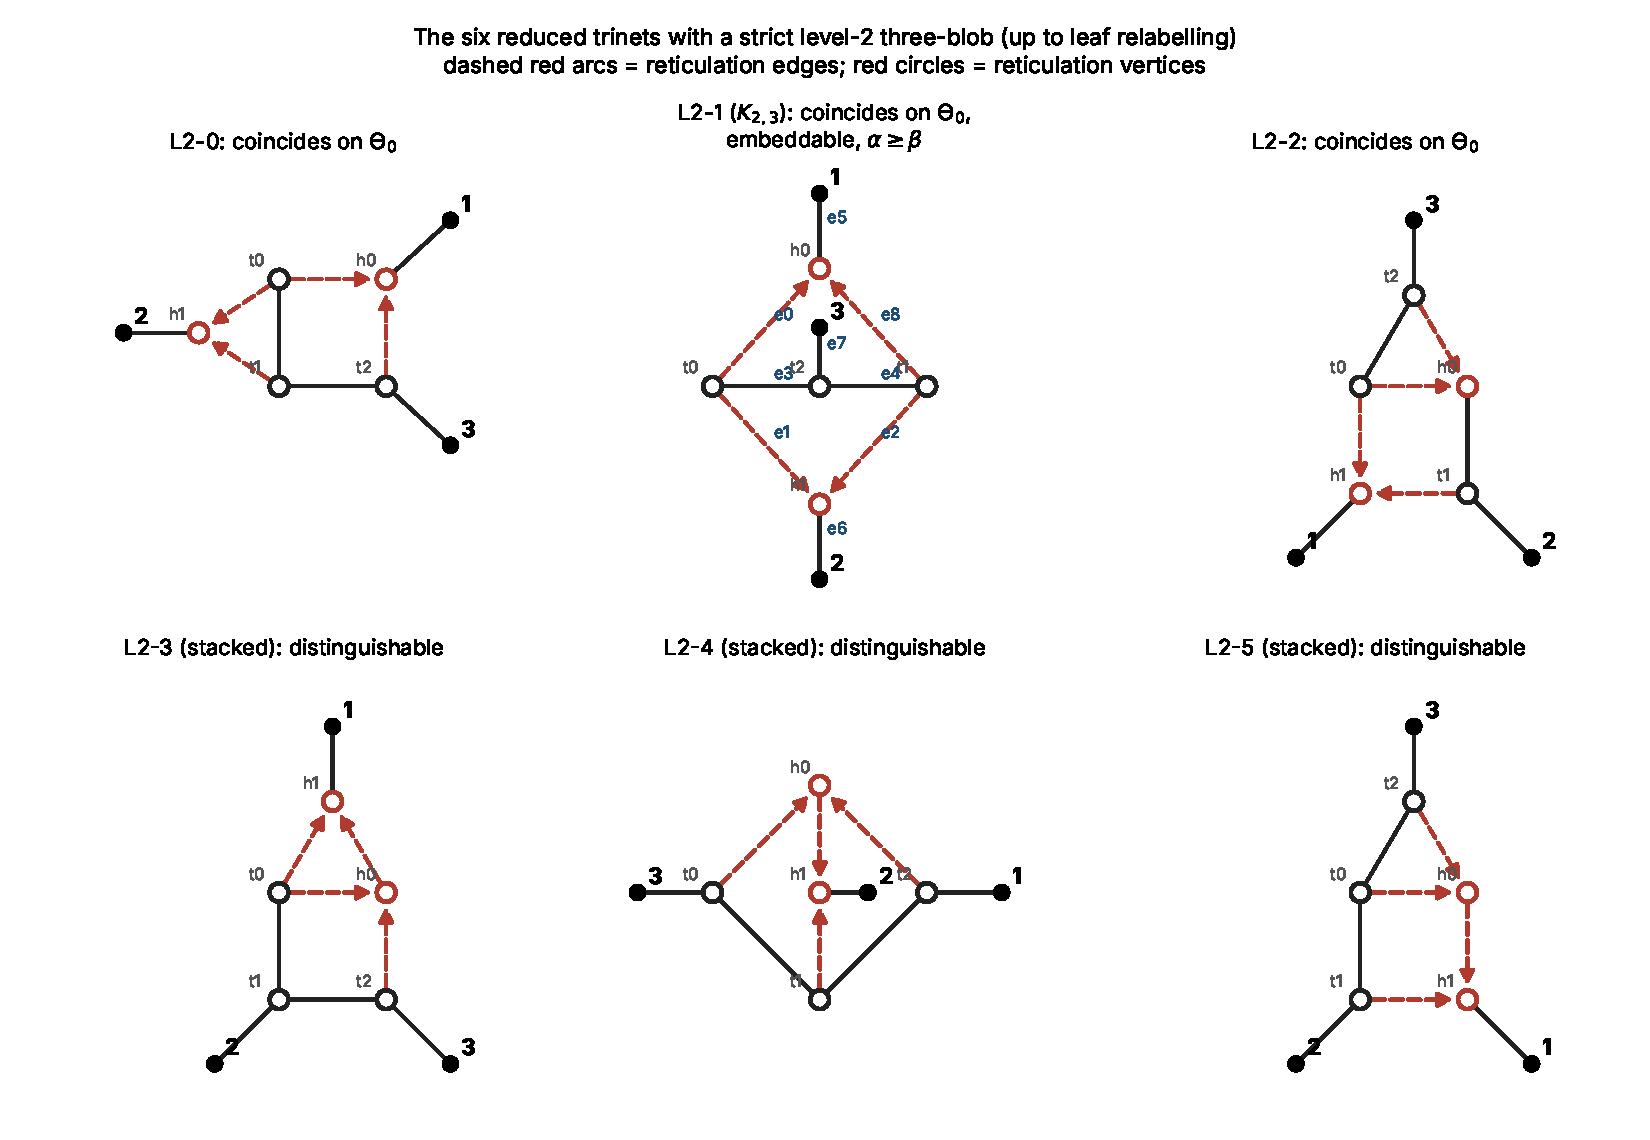
\includegraphics[width=1\linewidth,height=\textheight,keepaspectratio,alt={The six reduced trinets with a strict level-2 three-blob, up to relabelling of leaves. Dashed red arcs are reticulation edges and red circles reticulation vertices. Edge names e\_0,\textbackslash dots,e\_8 for L2-1 are those of Table 2.}]{../figures/fig1_level2_trinets.pdf}
\caption{The six reduced trinets with a strict level-2 three-blob, up to
relabelling of leaves. Dashed red arcs are reticulation edges and red
circles reticulation vertices. Edge names \(e_0,\dots,e_8\) for L2-1 are
those of Table 2.}
\end{figure}

\begin{table}[H]
\centering\small
\caption{Reduced level-two trinets. Coincidence is certified on $\Theta_0$ for the first three; only L2-1 is certified on $\Theta_{\rm tb}$. The two embeddable nonexistence entries remain conjectural. Every internal graph has cycle rank two.}
\begin{tabular}{llllll}
\toprule
Trinet & Reticulation leaves & Stacked & Anchored & $\Theta_0$ & $\Theta_{\rm emb}$\\
\midrule
L2-0 & 1, 2 & no & no & yes & open (Conj. 1)\\
L2-1 & 1, 2 & no & no & yes & yes\\
L2-2 & 1 & no & no & yes & open (Conj. 1)\\
L2-3 & 1 & yes & at 1 & no & no\\
L2-4 & 2 & yes & at 2 & no & no\\
L2-5 & 1 & yes & at 1 & no & no\\
\bottomrule
\end{tabular}
\end{table}

In L2-0 the triangle and the 4-cycle share a tree edge; in L2-2 the
triangle's reticulation lies on the 4-cycle.

\subsection{5. An exact counterexample}\label{an-exact-counterexample}

The trinet L2-1 has internal vertices \(t_0,t_1,t_2,h_0,h_1\). Both
reticulations \(h_0\) and \(h_1\) have parents \(t_0\) and \(t_1\); the
vertex \(t_2\) is joined to \(t_0\) and \(t_1\); leaves 1, 2 and 3 hang
from \(h_0\), \(h_1\) and \(t_2\). Its underlying graph is \(K_{2,3}\)
with parts \(\{t_0,t_1\}\) and \(\{t_2,h_0,h_1\}\). Placing the root on
the edge \(t_0t_2\) gives a valid rooted network.

\textbf{Theorem 1.} \emph{Give L2-1 the parameters of Table 2, with
mixing weight \(1/2\) at both reticulations. Its K2P leaf-pattern
distribution equals that of the star tree whose pendant edges to leaves
1, 2 and 3 have parameters}
\[(x_1,y_1)=\Bigl(\tfrac{\sqrt{105}}{396},\tfrac38\Bigr),\quad (x_2,y_2)=\Bigl(\tfrac{13\sqrt{105}}{900},\tfrac{3}{16}\Bigr),\quad (x_3,y_3)=\Bigl(\tfrac{\sqrt{105}}{70},\tfrac35\Bigr).\]
\emph{Every edge of both models lies in \(\Theta_{\mathrm{tb}}\); in
particular every edge matrix is stochastic, positive definite,
embeddable in continuous time, and has transition rate at least its
transversion rate.}

\begin{longtable}[]{@{}lllll@{}}
\caption{Parameters of the counterexample. \(\kappa=\alpha/\beta\) is
the transition/transversion rate ratio of the corresponding
continuous-time edge.}\tabularnewline
\toprule\noalign{}
Edge & Endpoints & \(X_e\) & \(Y_e\) & \(\kappa\) \\
\midrule\noalign{}
\endfirsthead
\toprule\noalign{}
Edge & Endpoints & \(X_e\) & \(Y_e\) & \(\kappa\) \\
\midrule\noalign{}
\endhead
\bottomrule\noalign{}
\endlastfoot
\(e_0\) & \(t_0 \to h_0\) & 31/990 & 464/1145 & 6.67 \\
\(e_1\) & \(t_0 \to h_1\) & 31/60 & 53/100 & 1.08 \\
\(e_2\) & \(t_1 \to h_1\) & 1/12 & 3/20 & 1.62 \\
\(e_3\) & \(t_2\) --- \(t_0\) & 51/155 & 1/2 & 2.21 \\
\(e_4\) & \(t_1\) --- \(t_2\) & 1/25 & 9/10 & 60.1 \\
\(e_8\) & \(t_1 \to h_0\) & 1/2 & 152/229 & 2.38 \\
\(e_5, e_6, e_7\) & pendant edges & 1/2 & 3/4 & 3.82 \\
\end{longtable}

\emph{Proof.} Choosing \(e_0\) or \(e_8\) at \(h_0\), and \(e_1\) or
\(e_2\) at \(h_1\), gives four displayed trees of weight \(1/4\) each.
Leaving aside the pendant edges, their paths from the meeting vertex to
leaves 1, 2, 3 are

{\def\LTcaptype{none} % do not increment counter
\begin{longtable}[]{@{}
  >{\raggedright\arraybackslash}p{(\linewidth - 6\tabcolsep) * \real{0.2500}}
  >{\raggedright\arraybackslash}p{(\linewidth - 6\tabcolsep) * \real{0.2500}}
  >{\raggedright\arraybackslash}p{(\linewidth - 6\tabcolsep) * \real{0.2500}}
  >{\raggedright\arraybackslash}p{(\linewidth - 6\tabcolsep) * \real{0.2500}}@{}}
\toprule\noalign{}
\begin{minipage}[b]{\linewidth}\raggedright
Displayed tree
\end{minipage} & \begin{minipage}[b]{\linewidth}\raggedright
Paths to leaves 1, 2, 3
\end{minipage} & \begin{minipage}[b]{\linewidth}\raggedright
\((X_1^T, X_2^T, X_3^T)\)
\end{minipage} & \begin{minipage}[b]{\linewidth}\raggedright
\((Y_1^T, Y_2^T, Y_3^T)\)
\end{minipage} \\
\midrule\noalign{}
\endhead
\bottomrule\noalign{}
\endlastfoot
\(e_0, e_1\) kept & \(e_0\); \(e_1\); \(e_3\) & (31/990, 31/60, 51/155)
& (464/1145, 53/100, 1/2) \\
\(e_0, e_2\) kept & \(e_0e_3\); \(e_2e_4\); --- & (17/1650, 1/300, 1) &
(232/1145, 27/200, 1) \\
\(e_8, e_1\) kept & \(e_8e_4\); \(e_1e_3\); --- & (1/50, 17/100, 1) &
(684/1145, 53/200, 1) \\
\(e_8, e_2\) kept & \(e_8\); \(e_2\); \(e_4\) & (1/2, 1/12, 1/25) &
(152/229, 3/20, 9/10) \\
\end{longtable}
}

By Lemma 2 the blob contributes
\[(A_1,A_2,A_3)=\Bigl(\tfrac{13}{150},\tfrac{1}{66},\tfrac{91}{5940}\Bigr),\quad (B_1,B_2,B_3)=\Bigl(\tfrac15,\tfrac25,\tfrac18\Bigr),\quad (C_1,C_2,C_3)=\Bigl(\tfrac{13}{300},\tfrac{1}{264},\tfrac{91}{7425}\Bigr).\]
With \((y_1,y_2,y_3)=(\tfrac12,\tfrac14,\tfrac45)\) these satisfy
\(B_1=y_2y_3\), \(B_2=y_1y_3\), \(B_3=y_1y_2\) and \(C_i = y_iA_i\) for
each \(i\), so \(E_1=E_2=E_3=0\). The pendant edges multiply \(A_i\) by
\(\tfrac14\), \(B_i\) by \(\tfrac{9}{16}\) and \(C_i\) by
\(\tfrac{3}{16}\), which leaves the binomials zero. Lemma 1 then gives
the star tree; its \(G\)-parameters are \(\tfrac34 y_i\), and
\(x_i = \tfrac12\sqrt{A_1A_2A_3}/A_i\) with
\(A_1A_2A_3 = 1183/58806000\), which yields the values stated. The edge
conditions are direct: for instance \(e_1\) has \(Y-X = 1/75 > 0\), and
the tree edge to leaf 2 has \(y_2^2 - x_2^2 = 9/256 - 1183/54000 > 0\).
\(\square\)

The 64 probabilities can be checked without relying on the Fourier
binomials. Computing each displayed tree's distribution from the
transition matrices by summing over all internal states, with exact
rational arithmetic, gives for example \(p_{AAA} = 1414811/60825600\)
and \(p_{ACG} = 693553/60825600\), and all 64 entries agree exactly with
those of the star tree. The star tree's probabilities are themselves
rational, because consistent Fourier-index patterns contain an even
number of the letters \(C,T\), so its \(x\)-parameters enter only in
pairs. Probability-space and Fourier calculations provide separate code
paths, not external peer review. The edge-specific rate ratios in Table
2 range from approximately 1.08 to 60.1: transition bias establishes
admissibility, not empirical typicality or a homogeneous process.

Three remarks place the example.

\emph{It refutes the withdrawn lemma directly.} That lemma asserted
\(E_x>0\) whenever leaf \(x\) lies below a reticulation of a trinet with
a non-trivial three-blob. Here \(E_1 = E_2 = 0\) at reticulation leaves
1 and 2.

\emph{It is not isolated.} The Jacobian of \((E_1,E_2,E_3)\) with
respect to the 20 network parameters has rank 3 at the point of Table 2,
computed exactly. The local coincidence locus is a smooth 17-dimensional
submanifold, hence has zero 20-dimensional Lebesgue measure locally. The
pendant edges rescale \(x_i\) and \(y_i\) freely while preserving zero
binomials, so the reproduced distributions nevertheless include a
non-empty open subset of the six-dimensional star-tree model. These are
different ambient spaces. Historical searches sampled \(400{,}000\) blob
vectors \((Y,\delta)\) and found completing \(X\) values for
approximately 27\%, 21\% and 15\% on the three regions respectively.
These are algorithm-dependent completion-search hit rates, not
full-network coincidence probabilities or certified volumes. The L2-1
and L2-2 routines scan 400 equally spaced values of \(t\) in
\([10^{-4},1]\) for \(X_3=t\,c(Y_3)\); L2-0 uses an algebraic inequality
test. These exploratory searches are not needed for the theorems.

\emph{It is a structured mixture, not an arbitrary one.} Mixtures can
mimic other trees (Matsen \& Steel, 2007; Štefankovič \& Vigoda, 2007;
Matsen et al., 2008). Allman et al.~(2012, Theorem 1) exclude mimicry
for certain single-tree mixtures with fewer components than states,
subject to a topology/refinement qualification; this is not a
prohibition on reproducing their own topology. Here four components
share edges and parameters as dictated by a network and reproduce the
three-leaf star. Kouwenhoven (2025, Chapters 4--5) had already studied
failure of a proposed K2P distinguishing polynomial; invariant failure
alone does not establish equality of all 64 probabilities. Our
certificate checks the latter. Sullivant's graphical-model equivalences
concern local network modifications and should not be confused with
equality to a tree model.

\subsection{6. Level two: which trinets coincide with
trees}\label{level-two-which-trinets-coincide-with-trees}

\textbf{Theorem 2.} \emph{On \(\Theta_0\), the trinets L2-0, L2-1 and
L2-2 each coincide with a star tree, and the trinets L2-3, L2-4 and L2-5
are distinguishable from every trinet without a non-trivial three-blob,
star trees included. The distinguishability holds on the whole box
\(0<X_e,Y_e<1\).}

\emph{Proof of the coincidences.} For L2-1 this is Theorem 1. For L2-0
and L2-2, Appendix A lists all-rational parameters in \(\Theta_0\), with
mixing weights \((4/5,1/2)\) and \((2/5,2/5)\), at which
\(E_1=E_2=E_3=0\) and the induced star-tree parameters lie in
\(\Theta_0\). The exact probability-space calculation again gives 64
identical entries in each case.

\emph{Proof of distinguishability.} Each of L2-3, L2-4 and L2-5 has a
reticulation \(h\) adjacent to a leaf \(x\) whose two parents are a tree
vertex \(p\) and another reticulation \(h'\). Deleting the edge
\(h'\to h\) leaves \(h'\) with no descendants, so the displayed network
is a star tree and \(E_x\) vanishes on it. Deleting the edge \(p\to h\)
leaves a 3-sunlet whose reticulation \(h'\) is adjacent to \(x\). For
the 3-sunlet with reticulation leaf \(x\), cycle tree edge \(f\) and
reticulation edges \(d,e\), a direct calculation gives
\[E_x = \delta(1-\delta)\,P\,X_f^2\,Y_dY_e\,(1-Y_f)^2,\] where \(P\) is
a product of parameters of the pendant edges, so \(E_x>0\) on the box
(this is Lemma 4.1 of Brits et al.). Theorem 3 below, applied with
anchor \(x\), completes the proof. A symbolic check confirms each step
for all three trinets. \(\square\)

The certificates for L2-0 and L2-2 use edge matrices outside
\(\Theta_{\mathrm{emb}}\): several edges have \(X_e^2 > Y_e\), so these
particular network points are not continuous-time embeddable. Their
comparison trees are embeddable. Whether all coincidences for these
shapes require non-embeddable network edges is unresolved. The
reductions in \texttt{feasibility\_regions.py} and
\texttt{rational\_search\_*.py} led to historical completion-search hit
rates of approximately 1.7\% and 2.2\% on \(\Theta_0\), and no hits on
\(\Theta_{\mathrm{emb}}\), in \(400{,}000\) sampled vectors. Searches
with 400 random starts approached boundary points. Neither search proves
nonexistence of an interior embeddable coincidence.

\textbf{Conjecture 1.} \emph{L2-0 and L2-2 are distinguishable from star
trees on \(\Theta_{\mathrm{emb}}\).}

The picture on continuous-time parameters is therefore different from
that on \(\Theta_0\), but the main conclusion does not depend on it:
L2-1 coincides with a tree even on \(\Theta_{\mathrm{tb}}\).

\subsection{7. Anchored trinets: a sufficient condition at every
level}\label{anchored-trinets-a-sufficient-condition-at-every-level}

Here is the Fourier action of the suppression used below. A degree-two
path replaces \((X_e,Y_e)\) by their coordinatewise products. A parallel
pair replaces them by a mixing-weighted coordinatewise mean. For a
two-interface sub-blob, condition on its internal reticulation choices
and sum out dangling parts. Each displayed tree contributes the product
of the Fourier edge parameters along the path between the interfaces,
with identity coefficient one. Thus the effective parameters are
positive weighted sums of path products, separately for \(X\) and \(Y\).
Include the two boundary edges in this effective path if necessary;
every path is then nonempty and its product is strictly between zero and
one. The same calculation applies when the root is trapped inside:
uniform-root group symmetry gives a two-interface kernel, and only
forward containment in the suppressed model is needed. Products and
convex means preserve the positive box and \(C/T\) symmetry even when
inverse Fourier entries are not nonnegative. This establishes the
forward-containment step on that box directly; it does not claim reverse
equality there or closure of the continuous-time region under mixtures.

The JC induction of Brits et al.~splits a trinet at a reticulation \(r\)
adjacent to a leaf \(x\). If \(e'\) and \(e''\) are the edges entering
\(r\) and \(\delta\) the weight of \(e'\), the displayed networks
\(N' = N - e''\) and \(N'' = N-e'\) satisfy
\[q = \delta\,q' + (1-\delta)\,q'' ,\] and the coordinates with state
\(A\) at leaf \(x\) (here \(A_x\) and \(B_x\)) are the same in \(q\),
\(q'\) and \(q''\) (Brits et al., Lemma 2.6). Expanding gives
\[E_x(q) = \delta^2E_x(q') + (1-\delta)^2E_x(q'') + \delta(1-\delta)\,K,\qquad K = A_x^2\bigl(B_j'B_k''+B_j''B_k'\bigr) - 2B_xC_x'C_x'' .\]
If \(E_x(q')\ge 0\) and \(E_x(q'')\ge0\), the inequality between
arithmetic and geometric means gives
\(K \ge 2A_x^2\sqrt{B_j'B_k'B_j''B_k''} - 2B_xC_x'C_x'' \ge 0\).
Everything turns on knowing \(E_x\ge0\) for the displayed networks,
\emph{at the same leaf \(x\)}. In those networks \(x\) may no longer lie
below a reticulation, and Section 5 shows that \(E_x\) can then be zero
or negative.

\textbf{Definition.} A reduced trinet \(N\) is \emph{anchored at leaf
\(x\)} if either \(N\) has no non-trivial three-blob, or \(x\) is
adjacent to a reticulation \(r\) of \(N\) and, for both edges \(e\)
entering \(r\), the displayed network \(N-e\) (with dangling parts
removed, vertices of degree two and parallel edges suppressed, and
2-sub-blobs suppressed) is anchored at \(x\).

\textbf{Theorem 3.} \emph{If a trinet \(N\) is anchored at \(x\), then
\(E_x \ge 0\) on the K2P model of \(N\) over the box \(0<X_e,Y_e<1\),
and \(E_x>0\) if \(N\) has a non-trivial three-blob. In that case \(N\)
is distinguishable from every trinet without a non-trivial three-blob,
on the box and hence on \(\Theta_0\).}

\emph{Proof.} We argue by induction on the number of reticulations.
Suppressing 2-sub-blobs, degree-two vertices and parallel edges does not
shrink a model (Brits et al., Lemma 5.1; for parallel edges and
degree-two vertices the box is closed under products and convex
combinations), so it suffices to treat reduced \(N\). If \(N\) has no
non-trivial three-blob it reduces to a star tree, on which
\(E_x \equiv 0\). Otherwise the expansion above applies at the
reticulation adjacent to \(x\). The points \(q'\) and \(q''\) lie in the
models of the reduced displayed networks, which are anchored at \(x\)
and have fewer reticulations, so \(E_x(q'), E_x(q'')\ge 0\) by
induction, \(K\ge0\), and \(E_x(q)\ge0\). For strictness: suppressing
2-sub-blobs does not destroy a non-trivial three-blob. A 2-sub-blob
\(W\) inside the blob contains at most one of the three vertices at
which the blob meets its outgoing edges: two of them would contribute
two leaving edges, and two more would join \(W\) to the rest of the
two-edge-connected blob. If one displayed network has a non-trivial
three-blob, its \(E_x\) is strictly positive by induction and enters
with a positive coefficient. If neither does, \(N\) has level one by
Lemma 5.4 of Brits et al., so it is a 3-sunlet with reticulation leaf
\(x\), and \(E_x>0\) by the formula in Section 6. Finally,
\(E_x\equiv0\) on every trinet without a non-trivial three-blob, by
Lemma 5.1 of Brits et al.~and Lemma 1. \(\square\)

The 3-sunlet is anchored at its reticulation leaf, and so are L2-3, L2-4
and L2-5 at the leaf below their lower reticulation. None of L2-0, L2-1,
L2-2 is anchored at any leaf: in each, every leaf below a reticulation
has a displayed network that is a 3-sunlet whose reticulation sits above
a \emph{different} leaf. That is precisely the configuration in which
the withdrawn induction step fails.

\subsection{8. Propagation, higher levels and more
leaves}\label{propagation-higher-levels-and-more-leaves}

Two operations carry a coincidence from small networks to larger ones.

\textbf{Lemma 4 (pendant subtrees).} \emph{If a trinet \(N\) and a star
tree \(S\) have the same distribution, attach rooted binary trees
\(T_1, T_2, T_3\) at the three leaves of both, with the same parameters.
The resulting \(n\)-leaf network and \(n\)-leaf tree have the same
distribution.}

\emph{Proof.} In every displayed tree, the states at the leaves of
\(T_i\) depend on the rest only through the state at the root of
\(T_i\), with the same conditional law in both models. Summing over the
three root states expresses both \(n\)-leaf distributions by the same
formula in terms of the common trinet distribution. \(\square\)

\textbf{Lemma 5 (one more reticulation).} \emph{Let \(N_0\) be a reduced
trinet that coincides with a star tree at a parameter point \(\theta_0\)
lying strictly inside a region
\(R \in \{\Theta_0, \Theta_{\mathrm{emb}}, \Theta_{\mathrm{tb}}\}\),
with strictly admissible star-tree parameters, at which the Jacobian of
\((E_1,E_2,E_3)\) has rank 3. Let \(N\) be any trinet with a
reticulation edge \(c\) such that \(N-c\), after removing dangling parts
and suppressing vertices of degree two and parallel edges (but no
2-sub-blob), is isomorphic to \(N_0\). Then \(N\) coincides with a star
tree at a point with the same three properties.}

\emph{Proof.} For an effective edge with interior parameters \((X,Y)\),
choose extra product factors strictly inside \(R\) and sufficiently
close to \((1,1)\), and divide \((X,Y)\) coordinatewise by their product
to obtain the remaining factor. Openness of strict admissibility keeps
that factor inside \(R\). Such near-identity factors exist in all three
regions, for example along a continuous-time path with rates
\(\alpha>\beta>0\). The derivatives with respect to the remaining \(X\)
and \(Y\) factors are the nonzero products of the extra factors, so this
product map has a local section and is a submersion. For parallel edges
use the same interior pair \((X,Y)\) on both edges, with a fixed mixing
weight in \((0,1)\). Their convex combination equals \((X,Y)\), and
varying one pair has nonzero scalar derivative in both coordinates. No
global convexity of the embeddable region is required: all individual
edge parameters remain in an open neighbourhood of the equal-pair
section. Compose these sections through the finite cleanup sequence;
disjoint effective edges have their own adjustable coordinates. Dangling
edges can be given arbitrary strictly interior parameters.

Write the lifted point as \(\widetilde\theta_0\). With \(\delta\) the
weight of the retained incoming edge, the coordinates are
\(q=\delta q_{N-c}+(1-\delta)q_{N-c'}\). At \((\widetilde\theta_0,1)\)
the residual map \(F=(E_1,E_2,E_3)\) vanishes and has rank-three
derivative in the old-edge directions because the cleanup map is a
submersion. The formula extends smoothly across this mixing-weight
boundary. Select a nonsingular three-column minor and apply the implicit
function theorem, fixing the other coordinates. It supplies solutions
for \(\delta<1\) sufficiently near one. Strict admissibility of every
edge, of the reconstructed tree (a continuous function of the positive
coordinates), and nonvanishing of the minor persist by openness.
\(\square\)

Lemma 5 needs some \(N\) to apply to. Given a reduced trinet with a
non-trivial three-blob, subdivide an edge of the blob by a new vertex
\(s\), subdivide the pendant edge of a leaf \(\ell\) by a new vertex
\(v\), and add the edge \(s\to v\). The result is a valid semi-directed
network, since \(v\)'s only descendant is \(\ell\). It is again reduced,
by a short case analysis on whether \(s\) and \(v\) belong to a putative
2-sub-blob (Appendix B), and its blob has one more reticulation.
Deleting \(s\to v\) returns the original. Iterating from L2-1, and then
attaching pendant subtrees, gives the main consequence.

\textbf{Corollary 6.} \emph{For every \(n\ge3\) and every \(k\ge2\)
there is an \(n\)-leaf network whose only non-trivial blob is a reduced
three-blob of level \(k\), and whose K2P model on
\(\Theta_{\mathrm{tb}}\) meets the model of an \(n\)-leaf binary tree.
Because a K2P edge with parameters \((X,Y)\) is a K3P edge with Fourier
parameters \((X,Y,X)\), the same holds for the K3P model on its space
\(\Theta_0\). Consequently the tree--network distinguishability theorem
of Brits et al.~(their Corollary 5.7) does not extend to K2P or K3P for
any number of leaves.}

Numerical continuation along Lemma 5 confirms the construction at levels
3 and 4. Starting from Theorem 1, with the new mixing weight lowered to
0.9, it reaches coincidence points at which the normalised binomials
\(\log(A_i^2B_jB_k)-\log(B_iC_i^2)\) are below \(10^{-14}\), with every
edge strictly inside \(\Theta_{\mathrm{tb}}\) and all mixing weights
between 0.49 and 0.93.

Lemma 5 also decides every level-3 trinet. Of the 83 reduced level-3
trinets, 30 are anchored and are therefore distinguishable by Theorem 3.
Each of the other 53 has a reticulation edge whose deletion leaves,
without any 2-sub-blob suppression, a copy of L2-0 (26 cases), L2-2 (21)
or L2-1 (6), counting the first such edge found. The certificates of
Theorems 1 and 2 are regular points strictly inside \(\Theta_0\), with
exactly computed Jacobian rank 3, so each of these 53 coincides with a
tree on \(\Theta_0\).

\textbf{Theorem 7 (classification up to level three;
computer-assisted).} \emph{A reduced trinet of level at most three with
a non-trivial three-blob is distinguishable from star trees on
\(\Theta_0\) if and only if it is anchored at some leaf.}

The enumerations behind Theorem 7 are computational, and the code is
part of the accompanying material. We have not enumerated level 4
exhaustively. Inserting one new reticulation edge, in every acyclic way,
into a rooted representative of each level-3 trinet produced 1,614
distinct reduced level-4 trinets. Of these, 443 are anchored and so
distinguishable. Each of the remaining 1,171 has a single deletion
leading to a non-anchored level-3 trinet, so by Lemma 5 each coincides
with a tree.

\textbf{Conjecture 2.} \emph{For every level, a reduced trinet with a
non-trivial three-blob is distinguishable from star trees on
\(\Theta_0\) under K2P if and only if it is anchored at some leaf.}

The anchored counts are 1 of 1, 3 of 6 and 30 of 83 in the exhaustive
classifications through level three. The 443 of 1,614 figure at level
four describes only the specified insertion-generated family; it is
neither an exhaustive count nor an unbiased estimate of the fraction
among all level-four trinets. Level-four and continuation outputs remain
exploratory historical evidence, not part of the exact
finite-classification gate.

On \(\Theta_{\mathrm{emb}}\) the picture is less complete. Fourteen
level-3 trinets contain a copy of L2-1 in the sense of Lemma 5, so they
coincide with trees even on \(\Theta_{\mathrm{tb}}\). One further
level-3 trinet does not contain L2-1 but still appears to coincide on
\(\Theta_{\mathrm{emb}}\). In it, all three reticulations lie above
leaves and share parents in a hexagon around a central tree vertex
(index 5 in the data files). A Newton refinement carried to 50
significant digits reduces \(|E|\) to \(10^{-57}\), with every
inequality satisfied by a margin of at least 0.027. This is numerical
evidence, not a certificate.

\subsection{9. Why JC and K2P behave
differently}\label{why-jc-and-k2p-behave-differently}

Lemma 2 shows what is at stake. The star tree's \(G\)-parameters \(y_i\)
are fixed by the pairwise coordinates \(B_i\). Coincidence then requires
each \(y_i\) to equal a weighted mean of the path values \(Y_i^T\) over
displayed trees, with weights proportional to \(w_TX_j^TX_k^T\).

Under JC every \(X_e\) equals \(Y_e\), so the weights are made from the
same numbers as the path values and the pairwise coordinates, and Brits
et al.'s inequality shows that the mean always falls short. Under K2P
the \(X_e\) are free, so the weights can be tuned independently of the
\(Y\) values. Coincidence requires two things: each \(y_i\) must lie
strictly between the smallest and largest path value \(Y_i^T\), and the
three sets of weights, which share the same \(X_e\), must be tunable at
the same time.

Anchoring describes when tuning is impossible. For the reticulation leaf
\(x\) of a 3-sunlet, both displayed trees give the same product
\(X_j^TX_k^T\), namely the parameter of the cycle's tree edge. The
weights are then exactly the mixing weights \((\delta,1-\delta)\), and
the JC inequality survives. In L2-1, by contrast, leaf 1 sees the four
displayed trees with \(X_2^TX_3^T \in \{X_1X_3, X_2X_4\}\), two products
whose ratio is free. In Theorem 1 the weights for leaf 1 are
proportional to \((51,1,51,1)\), and the weighted mean of the path
values \((464, 232, 684, 760)/1145\) is exactly \(y_1 = 1/2\). Leaves 2
and 3 are handled in the same way, and the remaining coupling between
the three weightings is one quadratic equation.

\subsection{10. Open questions}\label{open-questions}

\begin{enumerate}
\def\labelenumi{\arabic{enumi}.}
\tightlist
\item
  \emph{Continuous-time parameters.} Prove or refute Conjecture 1, and
  classify trinets on \(\Theta_{\mathrm{emb}}\); the level-3 example in
  Section 8 suggests that containing L2-1 is not the only route to
  coincidence there.
\item
  \emph{All levels.} Prove Conjecture 2. Theorem 3 gives one direction.
  For the other, it would suffice to show that every non-anchored trinet
  of level \(k\ge 3\) has a single reticulation-edge deletion leading,
  without 2-sub-blob suppression, to a non-anchored trinet of level
  \(k-1\). This holds for all 83 level-3 trinets and all 1,614 level-4
  trinets generated here.
\item
  \emph{Shared rate ratios.} Three questions differ: both models share
  the same prescribed ratio; each uses its own constant ratio; or only
  the network has a constant ratio and the tree is edge-specific.
  Proposition 8 below excludes the first for L2-1 when \(\kappa>1\). The
  second remains open. The historical \texttt{homogeneous\_kappa.py}
  search constrained only the network and did not check tree
  admissibility, so its \(\kappa=10\) residual hit is not an admissible
  certificate. The revised script checks reconstructed-tree
  admissibility and labels any output as numerical, network-only
  evidence. We do not rely on the historical hit.
\item
  \emph{K3P.} Since L2-3's model is contained in that of a 3-sunlet, the
  K3P level-1 result of Brits et al.~(their Lemma 4.2) makes L2-3
  distinguishable under K3P. The K3P status of L2-4 and L2-5 is open,
  because no single K3P binomial plays the role of \(E_x\).
\item
  \emph{Level-2 identifiability.} Englander et al.~(2025, bioRxiv
  version 1) establish JC identifiability under additional structural
  hypotheses. We do not transfer its theorem numbering across versions
  or infer a failure of generic identifiability from an exceptional
  coincidence. Theorem 2 blocks an unrestricted K2P trinet-separation
  argument on \(\Theta_0\). Restrictions on parameters or additional
  four-leaf information remain possible routes. Holtgrefe et al.~(2025)
  study quartet and inter-taxon quartet-distance information under
  specified structural assumptions; their data representation and
  question differ from the full-distribution coincidence here.
\end{enumerate}

\textbf{Proposition 8 (a common prescribed ratio).} \emph{L2-1 cannot
coincide with a tree if every edge of both models has the same fixed
transition/transversion ratio \(\kappa>1\), positive branch lengths and
strictly positive mixing weights.}

\emph{Proof.} Put \(r=(\kappa+1)/2>1\) and \(u_e=Y_e\), so
\(X_e=Y_e^r\). For each leaf pair \((j,k)\) let \(z_T=Y_j^TY_k^T\).
Lemma 2 gives \(A_i=\sum_Tw_Tz_T^r\) and \(B_i=\sum_Tw_Tz_T\). A tree
with this ratio requires \(A_i=B_i^r\). Strict convexity and positive
weights force all \(z_T\) equal for each pair. Removing common pendant
factors, the four path triples are \[
(u_0,u_1,u_3),\quad(u_0u_3,u_2u_4,1),\quad
(u_8u_4,u_1u_3,1),\quad(u_8,u_2,u_4).
\] The pair \((2,3)\) yields \(u_1u_3=u_2u_4\), whereas the pair
\((1,2)\) from the first two triples yields \(u_1=u_2u_3u_4\). Since
parameters are positive, substitution gives \(u_3^2=1\), contradicting
\(0<u_3<1\). The case \(\kappa=1\) is JC and is already excluded by the
source theorem. Nothing here excludes two different globally constant
ratios or an edge-specific comparison tree. \(\square\)

\subsection{11. Data and code}\label{data-and-code}

The release command
\texttt{python\ code/verify\_release.py\ -\/-out\ NEW\_DIRECTORY} runs
exact probability comparison, derivative checks, class/isomorphism and
deletion-route checks, and semantic negative controls. Running it with
\texttt{python\ -O} retains the explicit scientific failure checks. It
writes only to the requested new output directory. Historical searches
are classified separately in \texttt{STATUS.json}; small residuals,
finite-grid searches and the generated level-four family are not
promoted to exact certificates.

For each seed, columns \((X_0,X_1,X_3)\) give the following exact
nonzero minors of \(D(E_1,E_2,E_3)\):

\[
\begin{aligned}
\mathrm{L2\!\!-0}:&\quad \frac{2595026403}{334164131840000000000000000},\\
\mathrm{L2\!\!-1}:&\quad \frac{4090396401}{152331838470225920000000000000},\\
\mathrm{L2\!\!-2}:&\quad \frac{3310125802246725372991063338838110186542339249007963}{115989187909236791426228030377417451155908198400000000000000000000000}.
\end{aligned}
\]

The retained machine receipt also gives a nonzero nine-column minor of
the nine-coordinate map at each seed. These finite exact computations
support regularity; they are not formal verification of the universal
propagation argument.

The accompanying bundle contains the exact certificates
(\texttt{certificates/*.json}, together with the exact network
distributions in \texttt{*\_result.json}) and the probability-space
verifier \texttt{certify.py}. It also contains the enumeration code
(\texttt{trinets.py}, \texttt{enumerate\_level3.py}), the symbolic K2P
model (\texttt{k2p\_model.py}), the anchoring test
(\texttt{anchoring.py}), the level-3 and level-4 analyses, the searches
and reductions referred to above, and logs of every run. The
certificates use exact rational arithmetic, with arithmetic in
\(\mathbb{Q}(\sqrt{P})\) for the star-tree parameters.

\subsection{References}\label{references}

\textbf{Source problem and identifiability of phylogenetic networks}

Ardiyansyah, M. (2021). \emph{Distinguishing level-2 phylogenetic
networks using phylogenetic invariants} {[}Preprint{]}. arXiv.
https://arxiv.org/abs/2104.12479

Brits, J., Holtgrefe, N., van Iersel, L., \& Martin, S. (2026). \emph{On
tree-network distinguishability and full identifiability of phylogenetic
networks} (Version 3) {[}Preprint{]}. arXiv.
https://doi.org/10.48550/arXiv.2607.12919

Englander, A., Frohn, M., Gross, E., Holtgrefe, N., van Iersel, L.,
Jones, M., \& Sullivant, S. (2025). \emph{Identifiability of
phylogenetic level-2 networks under the Jukes-Cantor model}
{[}Preprint{]}. bioRxiv. https://doi.org/10.1101/2025.04.18.649493

Gross, E., \& Long, C. (2018). Distinguishing phylogenetic networks.
\emph{SIAM Journal on Applied Algebra and Geometry, 2}(1), 72--93.
https://doi.org/10.1137/17M1134238

Gross, E., van Iersel, L., Janssen, R., Jones, M., Long, C., \&
Murakami, Y. (2021). Distinguishing level-1 phylogenetic networks on the
basis of data generated by Markov processes. \emph{Journal of
Mathematical Biology, 83}, Article 32.
https://doi.org/10.1007/s00285-021-01653-8

Hollering, B., \& Sullivant, S. (2021). Identifiability in phylogenetics
using algebraic matroids. \emph{Journal of Symbolic Computation, 104},
142--158. https://doi.org/10.1016/j.jsc.2020.04.012

Sullivant, S. (2026). Phylogenetic network models as graphical models.
\emph{Bulletin of Mathematical Biology, 88}(8), Article 136.
https://doi.org/10.1007/s11538-026-01695-3

Kouwenhoven, G. (2025). \emph{Identifiability of phylogenetic trinets}
{[}Bachelor thesis, TU Delft{]}, Chapters 4--5.
https://repository.tudelft.nl/file/File\_533b1802-6a2f-4320-bc51-9941bd9f7f3b

Holtgrefe, N., Allman, E. S., Baños, H., van Iersel, L., Moulton, V.,
Rhodes, J. A., \& Wicke, K. (2025). \emph{Distinguishing phylogenetic
level-2 networks with quartets and inter-taxon quartet distances} (arXiv
version 2). https://arxiv.org/abs/2507.17308v2

\textbf{Mixtures that mimic trees}

Allman, E. S., Rhodes, J. A., \& Sullivant, S. (2012). When do
phylogenetic mixture models mimic other phylogenetic models?
\emph{Systematic Biology, 61}(6), 1049--1059.
https://doi.org/10.1093/sysbio/sys064

Matsen, F. A., Mossel, E., \& Steel, M. (2008). Mixed-up trees: The
structure of phylogenetic mixtures. \emph{Bulletin of Mathematical
Biology, 70}(4), 1115--1139. https://doi.org/10.1007/s11538-007-9293-y

Matsen, F. A., \& Steel, M. (2007). Phylogenetic mixtures on a single
tree can mimic a tree of another topology. \emph{Systematic Biology,
56}(5), 767--775. https://doi.org/10.1080/10635150701627304

Štefankovič, D., \& Vigoda, E. (2007). Phylogeny of mixture models:
Robustness of maximum likelihood and non-identifiable distributions.
\emph{Journal of Computational Biology, 14}(2), 156--189.
https://doi.org/10.1089/cmb.2006.0126

\textbf{Substitution models and Fourier coordinates}

Evans, S. N., \& Speed, T. P. (1993). Invariants of some probability
models used in phylogenetic inference. \emph{The Annals of Statistics,
21}(1). https://doi.org/10.1214/aos/1176349030

Kimura, M. (1980). A simple method for estimating evolutionary rates of
base substitutions through comparative studies of nucleotide sequences.
\emph{Journal of Molecular Evolution, 16}(2), 111--120.
https://doi.org/10.1007/BF01731581

\newpage

\subsection{Appendix A. Certificates for L2-0 and
L2-2}\label{appendix-a.-certificates-for-l2-0-and-l2-2}

Edges are listed as in Figure 1. Pendant edges have \((X,Y)=(1/2,3/4)\)
in both certificates. All parameters lie strictly inside \(\Theta_0\),
and the exact Jacobian of \((E_1,E_2,E_3)\) has rank 3 at both points.

\textbf{L2-0} (reticulation \(h_0\) with parents \(t_0\), \(t_2\) and
weight \(4/5\) on \(t_0\to h_0\); reticulation \(h_1\) with parents
\(t_0\), \(t_1\) and weight \(1/2\) on \(t_0\to h_1\)):

{\def\LTcaptype{none} % do not increment counter
\begin{longtable}[]{@{}lll@{}}
\toprule\noalign{}
Edge & \(X\) & \(Y\) \\
\midrule\noalign{}
\endhead
\bottomrule\noalign{}
\endlastfoot
\(t_0\to h_0\) & 16/45 & 20/43 \\
\(t_0\to h_1\) & 10/21 & 1/20 \\
\(t_1\to h_1\) & 1/2 & 79/100 \\
\(t_1\) --- \(t_0\) & 21/44 & 1/5 \\
\(t_2\) --- \(t_1\) & 15/28 & 1/10 \\
\(t_2\to h_0\) & 1/2 & 7/43 \\
\end{longtable}
}

The induced star tree has \(y=(3/20,3/20,3/20)\) and
\(x\approx(0.1639, 0.1848, 0.2635)\), all in \(\Theta_0\).

\textbf{L2-2} (reticulation \(h_0\) with parents \(t_0\), \(t_2\) and
weight \(2/5\) on \(t_0\to h_0\); reticulation \(h_1\) with parents
\(t_0\), \(t_1\) and weight \(2/5\) on \(t_0\to h_1\)):

{\def\LTcaptype{none} % do not increment counter
\begin{longtable}[]{@{}lll@{}}
\toprule\noalign{}
Edge & \(X\) & \(Y\) \\
\midrule\noalign{}
\endhead
\bottomrule\noalign{}
\endlastfoot
\(t_0\to h_0\) & 1572832833/1853838968 & 3/4 \\
\(t_0\to h_1\) & 1/5 & 80/141 \\
\(t_1\to h_1\) & 36588927/73906976 & 305/1692 \\
\(t_2\) --- \(t_0\) & 2197123/4619186 & 1/20 \\
\(h_0\) --- \(t_1\) & 3/4 & 3/4 \\
\(t_2\to h_0\) & 837103863/1853838968 & 11/72 \\
\end{longtable}
}

The induced star tree has \(y=(3/20,3/5,3/40)\) and
\(x\approx(0.1835,0.4429,0.1830)\), all in \(\Theta_0\).

\subsection{Appendix B. The one-arc extension keeps a trinet
reduced}\label{appendix-b.-the-one-arc-extension-keeps-a-trinet-reduced}

Let \(N\) be a reduced trinet whose internal vertices form a single
three-blob, and write \(\partial U\) for the number of edges joining a
set \(U\) of vertices to its complement.

\emph{Fact.} Every non-empty proper subset \(U\) of the internal
vertices of \(N\) has \(\partial U \ge 3\). If \(\partial U \le 1\), the
joining edge (if any) is a bridge, hence a pendant edge \(u\ell\), and
then the other two leaves are cut off from \(U\). If \(\partial U = 2\)
and \(U\) induces a connected subgraph, \(U\) is a 2-sub-blob or a
single vertex, which has degree three. If \(\partial U = 2\) and \(U\)
is disconnected, one of its components has \(\partial\le 1\).

Let \(N^+\) be obtained by subdividing a blob edge \(\{p,q\}\) with a
vertex \(s\) and the pendant edge \(\{u,\ell\}\) with a vertex \(v\),
and adding the arc \(s\to v\). Suppose \(W\) is a set of at least two
internal vertices of \(N^+\) that induces a connected subgraph and has
\(\partial W = 2\) in \(N^+\). In each case below we find a non-empty
proper subset of the internal vertices of \(N\) with \(\partial\le2\) in
\(N\), contradicting the Fact.

\begin{itemize}
\tightlist
\item
  \emph{Neither \(s\) nor \(v\) in \(W\).} If \(p,q\in W\), the edges
  \(ps\) and \(sq\) are the two leaving edges and \(\partial_N W = 0\).
  Otherwise the leaving edges of \(W\) in \(N^+\) correspond one-to-one
  with those in \(N\), so \(\partial_N W = 2\). In both cases \(W\) is
  proper, since the set of all internal vertices of \(N\) has five
  leaving edges in \(N^+\).
\item
  \emph{\(v\in W\), \(s\notin W\).} The edges \(v\ell\) and \(vs\) leave
  \(W\), so \(u\in W\) and nothing else leaves. Then \(W\setminus\{v\}\)
  has \(\partial_N = 1\).
\item
  \emph{\(s,v\in W\).} The edge \(v\ell\) leaves \(W\), and at most one
  further edge does. If \(u\notin W\), that edge is \(vu\), so
  \(p,q\in W\) and \(\partial_N(W\setminus\{s,v\}) = 0\). If \(u\in W\),
  then \(\partial_N(W\setminus\{s,v\}) \le 2\). The set
  \(W\setminus\{s,v\}\) is non-empty, because \(\{s,v\}\) alone has four
  leaving edges, and it is proper, because the set of all internal
  vertices of \(N^+\) has three leaving edges.
\item
  \emph{\(s\in W\), \(v\notin W\).} The edge \(sv\) leaves \(W\), and at
  most one further edge does, so \(\partial_N(W\setminus\{s\}) \le 1\).
  Here \(W\setminus\{s\}\) is non-empty because \(|W|\ge 2\).
\end{itemize}

Hence \(N^+\) has no 2-sub-blob. The vertices \(s\) and \(v\) lie on a
cycle through \(u\) and the old blob, so they join the blob, whose
number of reticulations rises by one. An orientation of \(N\) extends to
\(N^+\) without directed cycles, because \(v\)'s only descendant is
\(\ell\).

\end{document}
